%%%%%%%%%%%%%%%%%%%%%%%%%%%%%%%%%%%%%%%%%
% Beamer Presentation
% LaTeX Template
% Version 1.0 (10/11/12)
%
% This template has been downloaded from:
% http://www.LaTeXTemplates.com
%
% License:
% CC BY-NC-SA 3.0 (http://creativecommons.org/licenses/by-nc-sa/3.0/)
%
%%%%%%%%%%%%%%%%%%%%%%%%%%%%%%%%%%%%%%%%%

%----------------------------------------------------------------------------------------
%	PACKAGES AND THEMES
%----------------------------------------------------------------------------------------

\documentclass[10pt,handout]{beamer}
% \documentclass[10pt]{beamer}

\usepackage{fouriernc}
\usepackage{amsmath}
\usepackage{amssymb}
\usepackage{mathtools}
\usepackage{xcolor}
\usepackage[utf8]{inputenc}
\usepackage[T1]{fontenc}
\usepackage{textcase}
\usepackage{graphicx}

\mode<presentation> {

% The Beamer class comes with a number of default slide themes
% which change the colors and layouts of slides. Below this is a list
% of all the themes, uncomment each in turn to see what they look like.

%\usetheme{progressbar}
%\progressbaroptions{headline=sections}


% \usecolortheme{albatross}
\usecolortheme{beaver}
% \usecolortheme{beetle}
% \usecolortheme{crane}
% \usecolortheme{dolphin}
% \usecolortheme{dove}
% \usecolortheme{fly}
% \usecolortheme{lily}
% \usecolortheme{orchid}
% \usecolortheme{rose}
% \usecolortheme{seagull}
% \usecolortheme{seahorse}
% \usecolortheme{whale}
% \usecolortheme{wolverine}

%\setbeamertemplate{footline} % To remove the footer line in all slides uncomment this line
%\setbeamertemplate{footline}[page number] % To replace the footer line in all slides with a simple slide count uncomment this line

%\setbeamertemplate{navigation symbols}{} % To remove the navigation symbols from the bottom of all slides uncomment this line
}

\usepackage{graphicx} % Allows including images
\usepackage{booktabs} % Allows the use of \toprule, \midrule and \bottomrule in tables

\setbeamercovered{dynamic}
\definecolor{dgreen}{rgb}{0.,0.6,0.}
\newcommand{\beispiel}[1]{\textcolor{dgreen}{\textbf {#1}}}


%----------------------------------------------------------------------------------------
%	TITLE PAGE
%----------------------------------------------------------------------------------------

\title[RoBO]
{Robust Bayesian Optimization}
 % The short title appears at the bottom of every slide, the full title is only on the title page


\author{Joel Kaiser, José Luis Licón}
\institute[Uni Freiburg] % Your institution as it will appear on the bottom of every slide, may be shorthand to save space
{
Albert-Ludwigs-Universität Freiburg \\ % Your institution for the title page
\medskip
% \textit{liconj@informatik.uni-freiburg.de} % Your email address
}
\date{\today} % Date, can be changed to a custom date

\begin{document}
\setbeamertemplate{caption}{\insertcaption}



\begin{frame}
\titlepage % Print the title page as the first slide
\end{frame}

\begin{frame}
\frametitle{Overview} % Table of contents slide, comment this block out to remove it
\tableofcontents % Throughout your presentation, if you choose to use \section{} and \subsection{} commands, these will automatically be printed on this slide as an overview of your presentation
\end{frame}

%----------------------------------------------------------------------------------------
%	PRESENTATION SLIDES
%----------------------------------------------------------------------------------------

%------------------------------------------------
\section{Introduction}

%------------------------------------------------

\subsection{Bayesian Optimization}


%\begin{frame}
%\frametitle{Problem description}
% \begin{columns}[c]
  
% \column{.45\textwidth}

% \column{.6\textwidth}
% \begin{center}
% \scalebox{10}{\textbf{*}}
% \end{center}
% 
% \end{columns}

%\end{frame}

%------------------------------------------------

%------------------------------------------------

\subsection{Entropy Search}

\begin{frame}
\frametitle{Problem definition}

Let $I \subset \mathbb R^D$ be a bounded set, and $f : I \rightarrow \mathbb{R}$
a (possibly unknown) function. A probability measure $p(f)$ over the function
space $\mathbb{R}^I$ will in turn induce the following probability measure:

\[
	p_{min}(x) \coloneqq P \left\{ x = \arg\!\min f(x) \right\} = 
	\int_{f: I \rightarrow \mathbb{R}} p(f) \, 
		\prod_{\widetilde x \in I} H[f(\widetilde{x} - f(x)] df
\]

The objective will be to obtain a maximally informative probability measure
after a number $n$ of function evaluations. This problem is rendered 
computationally tractable by making several approximations. 
% \begin{columns}[c] % The "c" option specifies centered vertical alignment while the "t" option is used for top vertical alignment


% \column{.6\textwidth} % Right column and width

% \scalebox{10}{\textbf{*}}


\end{frame}

%------------------------------------------------
 
\begin{frame}
\frametitle{Problem definition}

\begin{itemize}
	\item $p(f)$ is defined as a Gaussian process
	\item $p_{min}$ is discretized to a set of representer points chosen from
	a non-uniform measure
	\item $p_{min}$ is approximated, either by expectation propagation
	or a Montecarlo method
	\item The change in $p(f)$ as a function of the next function evaluation
	can be predicted using the Gaussian process
	\item Relative entropy w.r.t. a uniform distribution is chosen as a loss
	function
	\item Expected information gain from future evaluations can be 
	approximated via the loss function
	\item The locations for new evaluations are evaluated greedily
\end{itemize}

\end{frame}

%------------------------------------------------
\section{RoBO}

\subsection{Architecture}

%------------------------------------------------
\begin{frame}
\frametitle{Main modules}
\begin{center}
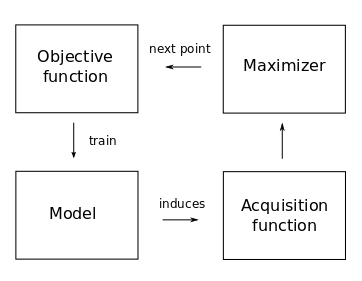
\includegraphics[width=0.7\textwidth]{robo_framework.png}
\end{center}

\end{frame}
%------------------------------------------------

%------------------------------------------------
\begin{frame}
\frametitle{Models}

Models are constructed as a wrapper to the GPy GPRegression class.

\begin{itemize}
\item Train (X,Z,Y), where Z are the instance features
\item marginalize features
\item conditionalize features
\item predict (X,Z) -> mean/variance
\item update(X,Z,Y)/downdate()
\item load / save functionality
\item Training should support approximations
\item Training should support an interface for optimizing the hyperparameters of the model
\item interface to compute the information gain
\item interface to draw sample from the model
\item validate()
\end{itemize}

\end{frame}
%------------------------------------------------

%------------------------------------------------
\begin{frame}
\frametitle{Acquisition functions}

\begin{itemize}
\item \textit{Expected Improvement}. Returns derivatives.
\item \textit{log(EI)}. Supports only one dimensional inputs, returns derivatives.
\item \textit{Probability of improvement}. Returns derivatives.
\item \textit{Upper confidence bound}. Not well tested.
\item \textit{Entropy Search}. EP-based information gain of the probability distribution
of the minimum.
\item \textit{Entropy MC}. Sample-based information gain of the probability distribution
of the minimum. Not yet stable.

\end{itemize}

\end{frame}
%------------------------------------------------

%------------------------------------------------
\begin{frame}
\frametitle{Other framework features}

\begin{itemize}
\item Support different kinds of parameters (conditional, categorial, 
continuous).
\item Can accept data set size as parameter.
\item REMBO
\item Can change model if the current one performs poorly
\item Chooser: can access history, predictions can be forwarded
\item Visualization is implemented for models and acquisition functions

\end{itemize}

\end{frame}
%------------------------------------------------


\subsection{Entropy Search Acquisition Function}
%------------------------------------------------




%------------------------------------------------



%------------------------------------------------
\section{Empirical Findings}

%\subsection{Test Functions}			

%------------------------------------------------




%------------------------------------------------
\subsection{Test Functions}
\begin{frame}
\frametitle{Data}
\begin{minipage}{0.55\textwidth}
Objective functions:
\begin{itemize}
\item Branin function
\begin{itemize}
\item dimensions: 2
\item global minima: 3
\item runs: 200
\end{itemize}
\item Self constructed test function
\end{itemize}
Used different acquisition funktion:
\begin{itemize}
\item Expected Improvement
\item Probability of improvement
\item Upper confidence bound
\item Entropy (Expectation Propagation)
\item Entropy (Monte Carlo)
\end{itemize}
\end{minipage}
\begin{minipage}[t]{0.43\textwidth}
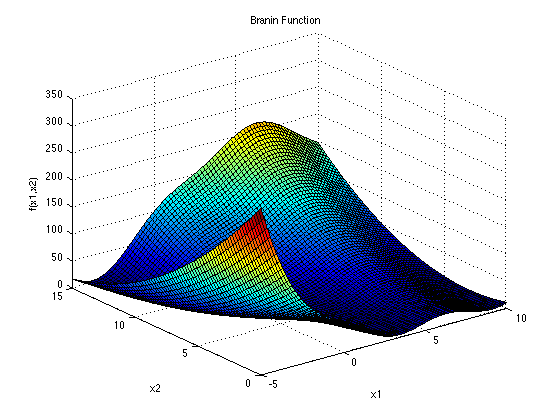
\includegraphics[width=\textwidth]{branin.png}
\end{minipage}
\end{frame}

%------------------------------------------------

\subsection{Results}

%------------------------------------------------
\begin{frame}
\frametitle{Results}
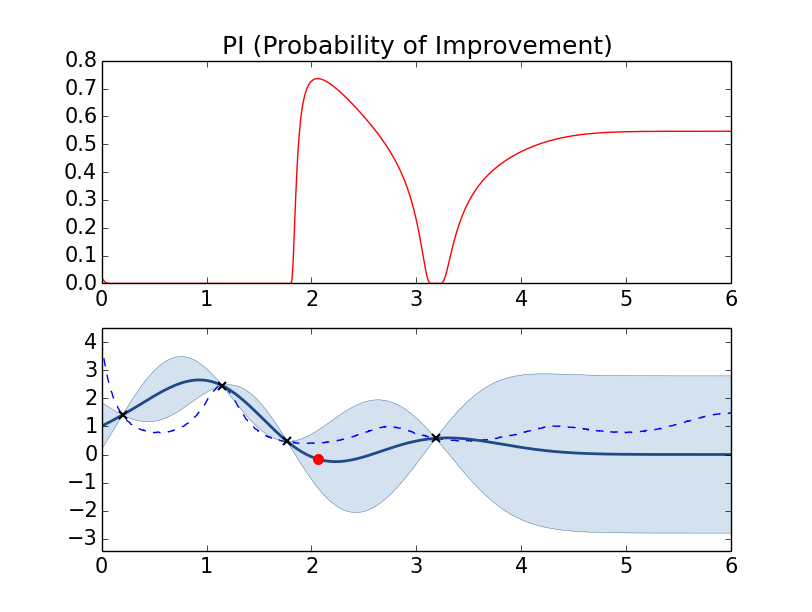
\includegraphics[width=\textwidth]{PI.png}
\end{frame}

%------------------------------------------------
\begin{frame}
\frametitle{Results}
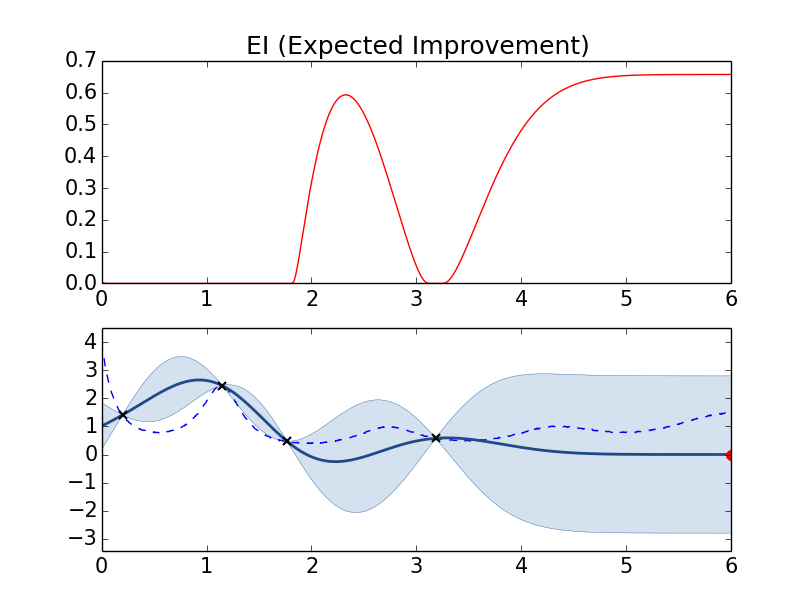
\includegraphics[width=\textwidth]{EI.png}
\end{frame}
%------------------------------------------------
\begin{frame}
\frametitle{Results}
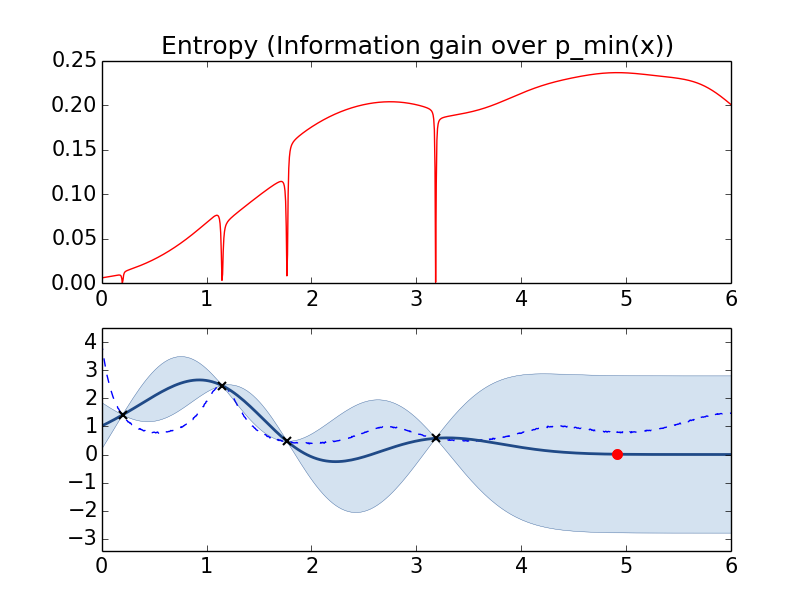
\includegraphics[width=\textwidth]{Entropy.png}
\end{frame}
%------------------------------------------------
\begin{frame}
\frametitle{Results}
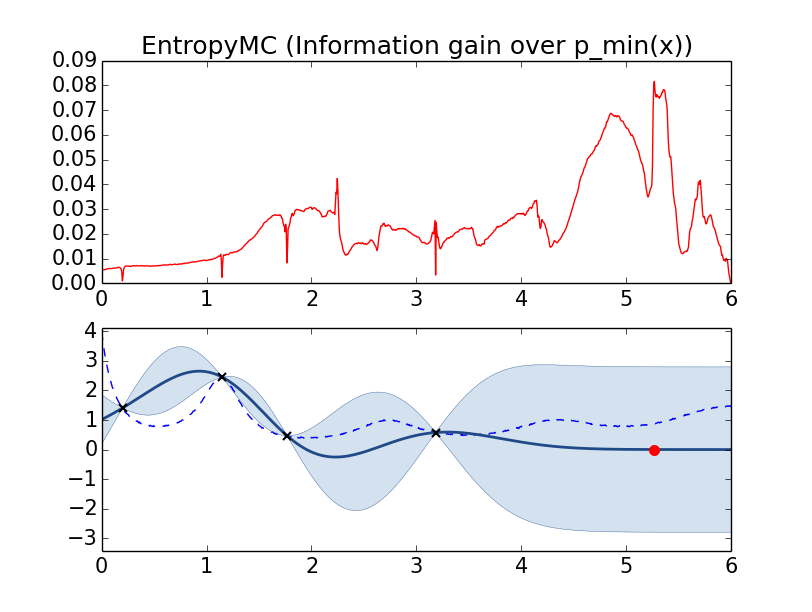
\includegraphics[width=\textwidth]{EntropyMC.png}
\end{frame}
%------------------------------------------------
\begin{frame}
\frametitle{Results}
 
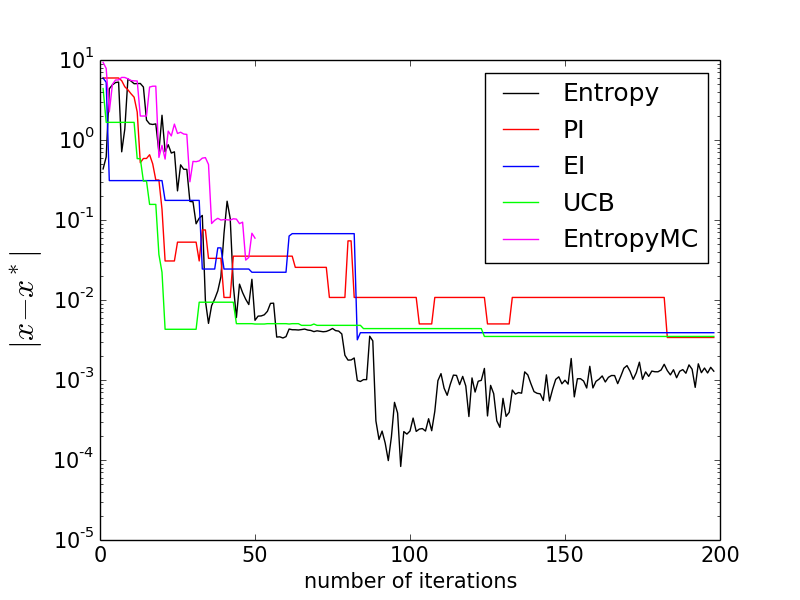
\includegraphics[width=\textwidth]{plot_branin2.png}

\end{frame}
%------------------------------------------------


%------------------------------------------------
\begin{frame}
\frametitle{Results}
 
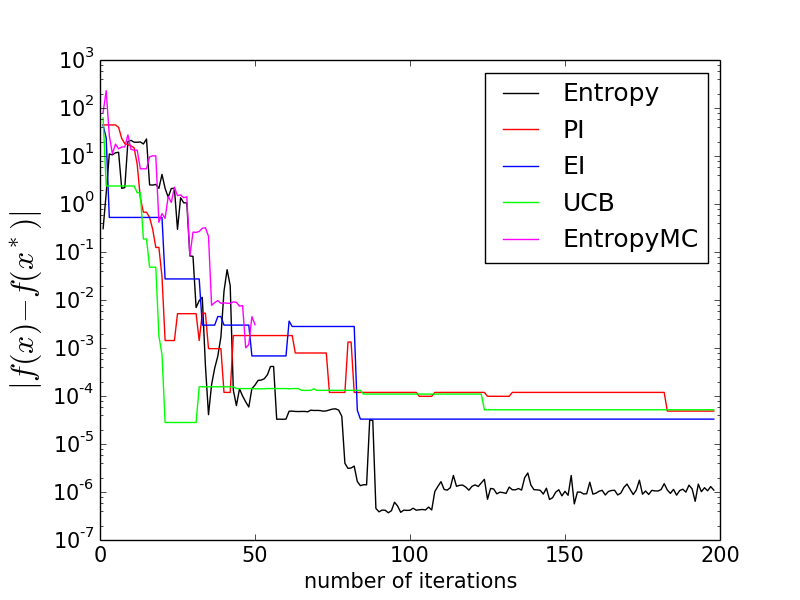
\includegraphics[width=\textwidth]{plot_branin1.png}

\end{frame}
%------------------------------------------------


%------------------------------------------------

\section{Conclusions}


%------------------------------------------------
\begin{frame}
\frametitle{Remarks}

\begin{itemize}[<+->]
	\item +
	\item -

\end{itemize}


\end{frame}


%------------------------------------------------
\begin{frame}
\frametitle{Future Directions}

\begin{itemize}
	\item EntropyMC
\end{itemize}

\end{frame}


%------------------------------------------------
%
%\begin{frame}
%\frametitle{References}
%\footnotesize{
%\begin{thebibliography}{99} % Beamer does not support BibTeX so references must be inserted manually as below
%%%%
%\bibitem[Hennig, 2011]{p1} Hennig, P.; Schuler, C. (2011)
%\newblock Entropy Search for Information-Efficient Global Optimization
%\newblock \emph{Proceedings of the Seventh Annual Symposium on Combinatorial
%Search (SoCS 20104)}.
%%%%%
%%\bibitem[birattari, 2010]{p1} Birattari, M. et al (2010)
%%\newblock F-race and iterated f-race: An overview.
%%\newblock \emph{Experimental Methods for the Analysis of Optimization 
%%Algorithms. Springer. 311-336}
%%%%%

%
%\end{thebibliography}
%}
%\end{frame}

%------------------------------------------------

%------------------------------------------------

%\begin{frame}
%\begin{center}
%\scalebox{10}{\textbf{?}}
%\end{center}
%\end{frame}

%------------------------------------------------



\begin{frame}
\Huge{\centerline{The End}}

\end{frame}

%----------------------------------------------------------------------------------------

			\end{document}
